%%%%%%%%%%%%%%%%%%%%%%%%%%%%%%%%%%%%%%%%%
% Daily Laboratory Book
% LaTeX Template
% Version 1.0 (4/4/12)
%
% This template has been downloaded from:
% http://www.LaTeXTemplates.com
%
% Original author:
% Frank Kuster (http://www.ctan.org/tex-archive/macros/latex/contrib/labbook/)
%
% Important note:
% This template requires the labbook.cls file to be in the same directory as the
% .tex file. The labbook.cls file provides the necessary structure to create the
% lab book.
%
% The \lipsum[#] commands throughout this template generate dummy text
% to fill the template out. These commands should all be removed when 
% writing lab book content.
%
% HOW TO USE THIS TEMPLATE 
% Each day in the lab consists of three main things:
%
% 1. LABDAY: The first thing to put is the \labday{} command with a date in 
% curly brackets, this will make a new page and put the date in big letters 
% at the top.
%
% 2. EXPERIMENT: Next you need to specify what experiment(s) you are 
% working on with an \experiment{} command with the experiment shorthand 
% in the curly brackets. The experiment shorthand is defined in the 
% 'DEFINITION OF EXPERIMENTS' section below, this means you can 
% say \experiment{pcr} and the actual text written to the PDF will be what 
% you set the 'pcr' experiment to be. If the experiment is a one off, you can 
% just write it in the bracket without creating a shorthand. Note: if you don't 
% want to have an experiment, just leave this out and it won't be printed.
%
% 3. CONTENT: Following the experiment is the content, i.e. what progress 
% you made on the experiment that day.
%
%%%%%%%%%%%%%%%%%%%%%%%%%%%%%%%%%%%%%%%%%

%----------------------------------------------------------------------------------------
%	PACKAGES AND OTHER DOCUMENT CONFIGURATIONS
%----------------------------------------------------------------------------------------

\documentclass[idxtotoc,hyperref,openany,oneside]{files/crypto} % 'openany' here removes the gap page between days, erase it to restore this gap; 'oneside' can also be added to remove the shift that odd pages have to the right for easier reading

\usepackage[ 
  backref=page,
  pdfpagelabels=true,
  plainpages=false,
  colorlinks=true,
  bookmarks=true,
  pdfview=FitB]{hyperref} % Required for the hyperlinks within the PDF
  
\usepackage{booktabs} % Required for the top and bottom rules in the table
\usepackage{float} % Required for specifying the exact location of a figure or table
\usepackage{graphicx} % Required for including images2
\usepackage{listings} % Used for programs' listings
\usepackage{tcolorbox} % For textboxes
\usepackage{amsmath} % For equation

\usepackage[english,russian]{babel}
\usepackage[utf8]{inputenc}
\usepackage [T2A] {fontenc}

\newcommand{\HRule}{\rule{\linewidth}{0.5mm}} % Command to make the lines in the title page
\setlength\parindent{0pt} % Removes all indentation from paragraphs

%----------------------------------------------------------------------------------------
%	DEFINITION OF EXPERIMENTS
%----------------------------------------------------------------------------------------

\newexperiment{easy1}{Based task}
\newexperiment{easy2}{Hashes among us}
\newexperiment{medium1}{Please be careful with ASR}
\newexperiment{medium2}{Please don't share}
\newexperiment{hard1}{Do you want to play some gamel?}
\newexperiment{hard2}{Curve task}

%---------------------------------------------------------------------------------------

\begin{document}

%----------------------------------------------------------------------------------------
%	TITLE PAGE
%----------------------------------------------------------------------------------------

\frontmatter % Use Roman numerals for page numbers
\title{
\begin{center}
\HRule \\[0.4cm]
{\Huge \bfseries CTF Code \\[0.5cm] \Large Writeups}\\[0.4cm] % Degree
\HRule \\[1.5cm]
\end{center}
}
\author{\Huge Криптография \\ \\[2cm]} % Your name and email address
\maketitle

\tableofcontents

\mainmatter % Use Arabic numerals for page numbers

%----------------------------------------------------------------------------------------
%	LAB BOOK CONTENTS
%----------------------------------------------------------------------------------------

% Blank template to use for new days:

%\labday{Day, Date Month Year}

%\experiment{}

%Text

%-----------------------------------------

%\experiment{}

%Text

%----------------------------------------------------------------------------------------

\labday{Easy}

\experiment{easy1}

\textbf{Теги:} baseN, googling\vspace{\baselineskip}

\begin{tcolorbox}
<условие задачи>
\end{tcolorbox}

Достаточно простая задача. Нам дается файл с какими-то иероглифами:
\begin{figure}[H]
\begin{center}

\includegraphics[width=1.0\linewidth]{files/chinese}
\end{center}
\caption{Китайцы уже близко}
\label{fig:chinese}
\end{figure}
Казалось бы, что тут можно придумать, переводчик выдает какую-то дичь. Если заметить название таска, то можно подумать про какую-то кодировку из base'ов. Немного гуглинга и можно наткнуться на весьма интересную штуку под названием \href{https://github.com/qntm/base65536}{base65536}. Прогнав через него натыкаемся на какую-то случайную последовательность эмодзи:
\begin{figure}[H]
\begin{center}

\includegraphics[width=1.0\linewidth]{files/emoji}
\end{center}
\caption{Кто-то слишком эмоционален}
\label{fig:emoji}
\end{figure}
Погуглив еще немного можно найти \href{https://github.com/AdamNiederer/base100}{base100}, после извлечения из которого получаем старый-добрый base64:
\begin{figure}[H]
\begin{center}
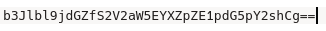
\includegraphics[width=0.7\linewidth]{files/base64}
\end{center}
\caption{То, что знакомо почти всем}
\label{fig:base64}
\end{figure}
И тут два варианта:
\begin{itemize}
\item Прогнать обратно ручками
\item Написать питоновский скрипт
\end{itemize}
Чтобы райтап был полным, рассмотрим второй вариант, потому что первый достаточно очевидный и не требует пояснений. Скрипт для расшифровки выглядит примерно следующим образом:
\begin{lstlisting}[language=Python, caption=Дешифровка флага]
#!/usr/bin/env python3
# -*- coding: utf-8 -*-

import base65536
import pybase100 as base100
import base64


def decode(flag):
    flag = base65536.decode(flag)
    flag = base100.decode(flag)
    flag = base64.b64decode(flag)
    flag = flag.decode('utf-8')

    return flag

def main():
    with open("flag.enc", 'r') as flag_file:
        flag = flag_file.read()

    print(flag)


if __name__ == '__main__':
    main()
\end{lstlisting}

На выходе получаем флаг \verb|oren_ctf_KevinDavidMitnick!|.

%-----------------------------------------

\experiment{easy2}

\textbf{Теги:} hash, hash crack\vspace{\baselineskip}

\begin{tcolorbox}
<условие задачи>
\end{tcolorbox}

Судя по виду зашифрованного флага и названию задачи перед нами какой-то хэш.
\begin{figure}[H]
\begin{center}
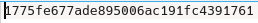
\includegraphics[width=1.0\linewidth]{files/md5flag}
\end{center}
\caption{Слишком много хексов}
\label{fig:chinese}
\end{figure}
Если посмотреть длинну, то мы увидим, что длинна флага ровно 32 символа, что позволяет подумать про MD5. Дальше можно либо брутить локально с помощью HashCat/JhonTheRipper или воспользоваться онлайн-сервисами наподобие \href{https://crackstation.net/}{CrackStation}. После чего получаем строку \verb|RobertMorris|, которую нужно обернуть в \verb|oren_ctf_| и \verb|!|. После чего получаем флаг \verb|oren_ctf_RobertMorris!|.

%----------------------------------------------------------------------------------------

\labday{Medium}

\experiment{medium1}

\textbf{Теги:} RSA, Hastad Attack\vspace{\baselineskip}

\begin{tcolorbox}
<условие задачи>
\end{tcolorbox}

Судя по ключам и названию задчи речь явно идет про RSA. Что же, можно погуглить про атаки на этот алгоритм и наткнуться на весьма интересную штуку под названием \href{https://en.wikipedia.org/wiki/Coppersmith\%27s_attack#H\%C3\%A5stad's_broadcast_attack}{Håstad's broadcast attack}. После чего, если попробовать сдампить открытую экспоненту и модуль из наших открытых ключей, то можно увидеть, что во всех трех ключах экспонента маленькая и равна 3. Что уже точно намекает на эту атаку. 

\textbf{Суть атаки}

Пользователь $А$ отсылает зашифрованное сообщение m нескольким пользователям. в данном случае, трём (по числу файлов): $P1$, $P2$, $P3$. У каждого пользователя есть свой ключ, представляемый парой «модуль-открытая экспонента» ($n_i$, $e_i$), причём $M < n1$, $n2$, $n3$. Для каждого из трех пользователей $А$ зашифровывает сообщение на соответствующем открытом ключе и отсылает результат адресату.
Атакующий же реализует перехват сообщений и собирает переданные шифртексты (обозначим их как $C_1$, $C_2$, $C_3$), с целью восстановить исходное сообщение $M$. Значит, по имеющимся трем шифртекстам нужно восстановить сообщение, которое будет флагом.

\textbf{Почему точно сможем ее реализовать?}

Как известно, шифрование сообщения по схеме RSA происходит следующим образом: $C = M^e \pmod{n}$. В случае с открытой экспонентой, равной 3, получение шифртекстов выглядит так:
\begin{center}
$C_1 = M^3 \pmod{n_1}$

$C_2 = M^3 \pmod{n_2}$

$C_3 = M^3 \pmod{n_3}$
\end{center}
Зная, что $n_1$, $n_2$, $n_3$ взаимно просты, можем применить к шифртекстам \href{https://ru.wikipedia.org/wiki/\%D0\%9A\%D0\%B8\%D1\%82\%D0\%B0\%D0\%B9\%D1\%81\%D0\%BA\%D0\%B0\%D1\%8F_\%D1\%82\%D0\%B5\%D0\%BE\%D1\%80\%D0\%B5\%D0\%BC\%D0\%B0_\%D0\%BE\%D0\%B1_\%D0\%BE\%D1\%81\%D1\%82\%D0\%B0\%D1\%82\%D0\%BA\%D0\%B0\%D1\%85}{китайскую теорему об остатках}. Получим в итоге некоторое $C'$, корень кубический из которого и даст нам искомое сообщение $M$.
\begin{center}
$C' = M^3 \pmod{n_1*n_2*n_3}$
\end{center}
Вспоминаем, что $M$ меньше каждого из трёх модулей $n_i$, значит, справедливо равенство:
\begin{center}
$C' = M^3$
\end{center}
Так мы и найдем наше искомое сообщение $M$.

\textbf{Программная реализация атаки Хастада}

После всего вышесказанного не составляет труда написать простенький скрипт на питоне, который выдает зашифрованное сообщение:
\begin{lstlisting}[language=Python, caption=Атака Хастада]
#!/usr/bin/env python3
# -*- coding: utf-8 -*-

import gmpy2
gmpy2.get_context().precision = 2048

from binascii import unhexlify
from functools import reduce
from gmpy2 import root
from Crypto.PublicKey import RSA


def chinese_remainder_theorem(items):
    N = 1
    for a, n in items:
        N *= n

    result = 0
    for a, n in items:
        m = N // n
        r, s, d = extended_gcd(n, m)
        if d != 1:
            raise "Input not pairwise co-prime"
        result += a * s * m

    return result % N


def extended_gcd(a, b):
    x, y = 0, 1
    lastx, lasty = 1, 0

    while b:
        a, (q, b) = b, divmod(a, b)
        x, lastx = lastx - q * x, x
        y, lasty = lasty - q * y, y

    return (lastx, lasty, a)


def mul_inv(a, b):
    b0 = b
    x0, x1 = 0, 1
    if b == 1:
        return 1
    while a > 1:
        q = a // b
        a, b = b, a % b
        x0, x1 = x1 - q * x0, x0
    if x1 < 0:
        x1 += b0

    return x1


def get_cipher(filename):
    with open(filename, 'rb') as cipher:
        value = cipher.read().hex()

    return int(value, 16)


def get_modulus(filename):
    with open(filename) as keyfile:
        keystr = keyfile.read()
        key = RSA.import_key(keystr)

    return key.n


def main():
    ciphertext1 = get_cipher("flag.enc.alice")
    ciphertext2 = get_cipher("flag.enc.bob")
    ciphertext3 = get_cipher("flag.enc.eve")

    modulus1 = get_modulus("alice.pub")
    modulus2 = get_modulus("bob.pub")
    modulus3 = get_modulus("eve.pub")

    C = chinese_remainder_theorem([(ciphertext1, modulus1), 
    					(ciphertext2, modulus2),
    					(ciphertext3, modulus3)])
    flag = int(root(C, 3))
    flag = hex(flag)[2:]

    print(unhexlify(flag).decode('utf-8'), end='')


if __name__ == '__main__':
    main()
\end{lstlisting}

После выполнения скрипта на выходе получаем расшифрованный текст с флагом:
\begin{verbatim}
CIH, also known as Chernobyl or Spacefiller, is a Microsoft Windows 9x
computer virus which first emerged in 1998. Its payload is overwriting
critical information on infected system drives, and in some cases
destroying the system BIOS. Flag: oren_ctf_CIH!
\end{verbatim}

%-----------------------------------------

\experiment{medium2}

\textbf{Теги:} Shamir's Secret Sharing, AES\vspace{\baselineskip}

\begin{tcolorbox}
<условие задачи>
\end{tcolorbox}

При подключении к серверу мы видим сообщение
\begin{figure}[H]
\begin{center}
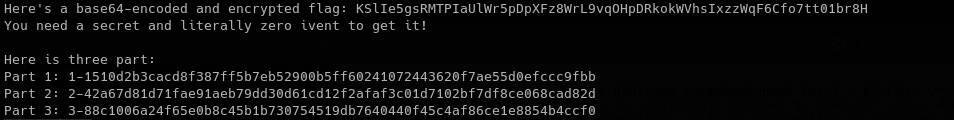
\includegraphics[width=1.0\linewidth]{files/shamir_aes}
\end{center}
\caption{Выглядит странно}
\label{fig:chinese}
\end{figure}
Исходя из названия задачи и формулировки подсказки можно предположить, что речь идет о \href{https://en.wikipedia.org/wiki/Shamir\%27s_Secret_Sharing}{Shamir Secret Sharing Scheme} (или иногда можно встретить сокращение SSSS). Помимо этого есть опечатка в слове \verb|event|, что тоже дает какую-то подсказку. По подсказке понятно, что схемой разбит не сам флаг, а ключ для какого-то алгоримта шифрования с нулевым вектором инициализации, которым уже зашифрован флаг.

\textbf{Немного о схеме Шамира}

Если очень кратко, то секрет (информация, которой мы хотим поделиться) $S$ разбивается на $n$ частей таким образом, чтобы можно было восстановить исходное сообщение $S$ только в случае, если мы имеем не менее $k$ кусочков из $n$. Даже наличие $k-1$ куска недостаточно, чтобы восстановить исходную $S$. Чуть более подробно про это написано вот \href{https://habr.com/ru/post/431392/}{здесь}.

\textbf{Реализация}

Можно писать разделение секрета самому, но это выходит за рамки данного райтапа. Если немного погуглить, то можно найти достаточно большое количество реализаций этого алгоритма на самых разных языках. Для питона существует вот \href{https://github.com/shea256/secret-sharing}{эта} реализация, но, к сожалению, она имеет проблемы с третьей версией из-за использования типа \verb|long|, который был удален. Но ничего не мешает написать скрипт на втором. Итак, после получения полного секрета можно заметить, что это строка длинной 16 символов, что, в купе с нулевым инициализирующим вектором, дает возможность предположить, что используется AES-128. Остается лишь понять, какой из двух самых известных вариантов используется - ECB или CBC. Это можно сделать просто попробовав каждый из них. После чего можно написать небольшой питоновский скрипт, чтобы получить флаг:
\begin{lstlisting}[language=Python, caption=Расшифровка флага AES-CBC]
#!/usr/bin/env python2
# -*- coding: utf-8 -*-

import sys
from base64 import b64decode
from Crypto.Cipher import AES
from secretsharing import SecretSharer


def main():
    if len(sys.argv) < 4:
        print("Usage: {} part1 part2 part2".format(sys.argv[0]))
        exit(1)

    AES_KEY = SecretSharer.recover_secret([sys.argv[1], sys.argv[2], sys.argv[3]])
    IV = b'\x00' * 16
    cipher = AES.new(key=AES_KEY, mode=AES.MODE_CBC, iv=IV)

    with open("flag.enc", 'r') as flagfile:
        enc_flag = b64decode(flagfile.read())

    flag = cipher.decrypt(enc_flag)

    print("Decrypted flag is: {}".format(flag))


if __name__ == '__main__':
    main()
\end{lstlisting}

После выполнения скрипта на выходе получаем расшифрованный флаг: 

\verb|Decrypted flag is: oren_ctf_ILOVEYOU_or_LoveLetter!|

%----------------------------------------------------------------------------------------

\labday{Hard}

\experiment{hard1}

\textbf{Теги:} Elgamal\vspace{\baselineskip}

\begin{tcolorbox}
<условие задачи>
\end{tcolorbox}

При подключении к серверу мы видим сообщение
\begin{figure}[H]
\begin{center}
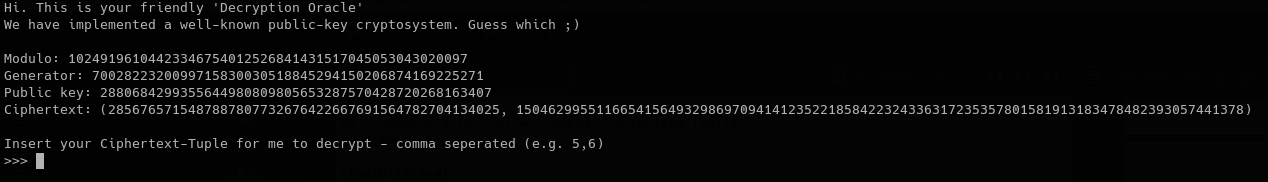
\includegraphics[width=1.0\linewidth]{files/elgamal}
\end{center}
\caption{Опять какая-то асимметрия}
\label{fig:chinese}
\end{figure}
Судя по тому, что шифротекст разделен на два числа - перед нами криптосистема Эль-Гамаля.

\textbf{Криптосистема Эль-Гамаля}

Идея данной системы основана на сложности нахождения целого неотрицательного числа $x$, удовлетворяющего уравнению $g^x = a$ в циклической группе\footnote{Тут нужно некоторое уточнение. Циклическая группа $(G, *)$, если не вдаваться в дебри высшей математики, - множество для элементов которого мы определили по каким правилам можно их складывать (строго говоря, то сложение которое проходят в школе и это - немного разные вещи. В данном случае под сложением подразумевается операция, которая однозначно ставит в соответствие двум элементам $e_1$ и $e_2$ группы $G$ некоторый элемент $e_3$, также принадлежащий группе $G$). Эта группа особенна тем, что результат операции может быть меньше операндов. По поводу цикличности все совсем просто - группа образуется некоторым элементом $g$, который называется образующим, а все остальные ее элементы это степени образующего. То есть $G = \{g^1, g^2, ...\}$. Группа становится циклической, если в $g^n = g$. Тогда число $n$ называется порядком группы.} (вообще говоря, такая операция называется дискретным логарифмированием). 

\textit{Генерация ключа}

Алгоритм генеарции ключа работает по следующему принципу:
\begin{itemize}
	\item Выбираем случайное большое целое число $q$ и строим циклическую группу $G_q$ с образующим элементом $g$.
	\item Выбираем случайный целочисленный положительный $x$, т. ч. $1 \leq x \geq q - 1$ и $НОД(x, q) = 1$
	\item Считаем $h = g^x$
	\item Публичный ключ состоит из трех частей: $(q, g, h)$
\end{itemize}

\textit{Шифрование}

Пусть мы хотим передать некоторое сообщение M. Тогда:
\begin{itemize}
	\item Выбирается случайный целочисленный положительный $y$, $1 \leq y \geq q - 1$ и $НОД(y, q) = 1$
	\item Вычисляется секрет $s = h^y = (g^x)^y = g^{xy}$
	\item Вычисляется $c_1 = g^y$
	\item Вычисляется $c_2 = M * s$
\end{itemize}
Шифротекстом будет пара $(c_1, c_2)$

\textit{Дешифровка}

Мы хотим расшифровать сообщение $(c_1, c_2)$ и у нас есть приватный ключ $x$. Если провести некоторые математические выкладки:
\begin{center}
\begin{equation*}
 \begin{cases}
   c_1 = g^y 
   \\
   c_2 = M * s
 \end{cases}
\end{equation*}
$\Rightarrow$
\begin{equation*}
 \begin{cases}
   c_1 = g^y 
   \\
   c_2 = M * h^y
 \end{cases}
\end{equation*}
$\Rightarrow$
\begin{equation*}
 \begin{cases}
   c_1 = g^y 
   \\
   c_2 = M * g^{xy}
 \end{cases}
\end{equation*}
\end{center}
То есть для получения оригинального сообщения M необходимо произвести следующие операции:
\begin{center}
$M = \frac{c_2}{c_1^y} = \frac{M * g^{xy}}{g^{xy}}$.
\end{center}

\textbf{Атака}

Очевидно, что тот же самый шифротекст система отказывается расшифровывать. Но можно немного схитрить - умножить и поделить дробь на два. От этого, как известно, результат не поменяется:
\begin{center}
$c_2' = c_2 * 2$

$M * 2 = \frac{c_2'}{c_1^y} = \frac{c_2 * 2}{c_1^y} = \frac{M * g^{xy} * 2}{g^{xy}}$.
\end{center}
После чего останется только поделить сообщение на два и получить флаг!

\textbf{Реализация}

После всего вышеперечисленного написать простенький скрипт на питоне не составляет труда. Для упрощения самому себе жизни я буду использовать библиотеку \verb|pwntools| (вообще говоря, она задумывалась для работы с бинарщиной, но также через нее весьма удобно работать с сокетами):
\begin{lstlisting}[language=Python, caption=Взлом криптосистемы Эль-Гамаля]
#!/usr/bin/env python3
# -*- coding: utf-8 -*-

from pwn import *
import re


def get_cipher(msg):
    str_tp = re.search(r'\d*, \d*', msg).group(0)

    return tuple(map(int, str_tp.split(', ')))


def mul_tuple(tuple):
    new_tuple = (tuple[0], tuple[1] * 2)

    return  ', '.join(map(str, new_tuple))


def get_decrypt_flag(enc_flag):
    hexflag2 = ''.join('{:02x}'.format(ord(ch)) for ch in enc_flag)
    numflag2 = int(hexflag2, 16)
    numflag = numflag2 // 2
    hexflag = hex(numflag)[2:]

    return ''.join([chr(int(''.join(ch), 16)) \ 
    		for ch in zip(hexflag[0::2], hexflag[1::2])])


def main():
    r = remote('localhost', 1488)

    msg = r.recvuntil('>>> ').decode('utf-8')
    tuple = get_cipher(msg)

    msg_for_flag = mul_tuple(tuple)
    r.sendline(msg_for_flag)

    enc_flag = r.recvline().decode('utf-8')
    flag = get_decrypt_flag(enc_flag)

    print("Decrypted flag: {}".format(flag))

    r.close()


if __name__ == '__main__':
    main()
\end{lstlisting}

На выходе скрипта получаем флга \verb|oren_ctf_WannaCry!|

%-----------------------------------------

\experiment{hard2}

\textbf{Теги:} Diffie-Hellman, Elliptic curve\vspace{\baselineskip}

\begin{tcolorbox}
<условие задачи>
\end{tcolorbox}

В задаче применяется алгоритм Диффи-Хеллмана, но немного усложненная версия на элептических кривых. Традиционная аббревиатура: ECDH (Elliptic Curve Diffie-Hellman). Подробнее про криптографию на элептических кривых можно почитать \href{https://habr.com/ru/post/335906/}{вот тут}. Нам дается клиент и сетевой дамп его общения с сервером.

Алгоритм клиента выглядит следующим образом:
\begin{itemize}
	\item Подключение к серверу и получение параметра кривой: $a$, $b$, $p$ (уравнение кривой выглядит как $y^2 = x^3 + a*x + b (\pmod{p})$).
	\item Получение начальной точки $G$
	\item Подтверждение начальной точки (или отказ от нее и предложение своей)
	\item Вычисление секретного ключа $a$ как случайного числа
	\item Отправка $G * a$
	\item Получение от сервера $G * d$ (где $d$ - секретный ключ сервера)
	\item Вычисление общего ключа $s = a * (dG) = adG$
\end{itemize}

Сессия выглядит следующим образом:
\begin{figure}[H]
\begin{center}
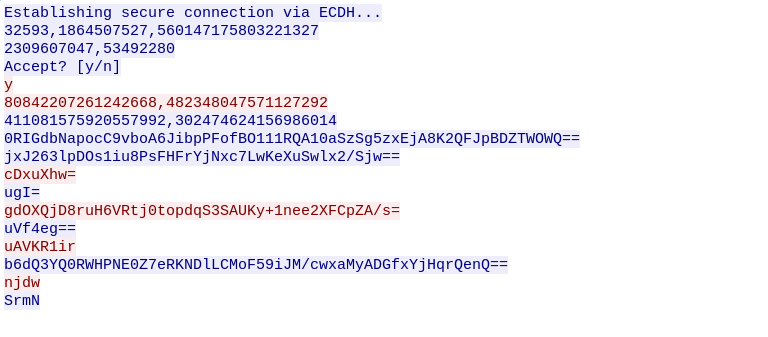
\includegraphics[width=1.0\linewidth]{files/wireshark}
\end{center}
\caption{Где-то здесь точно есть флаг}
\label{fig:chinese}
\end{figure}

Как можно заметить, модуль $p$ не очень большой: $560147175803221327$ это примерно 59 бит. Поэтому в данном случае заходит решение "в лоб"{} через вычисление дискретного логарифма (см. предыдущую задачу). Можно попробовать самому реализовать какой-то из вариантов, но проще всего использовать \href{https://www.sagemath.org/}{sage}:
\begin{figure}[H]
\begin{center}
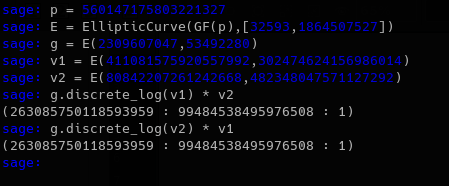
\includegraphics[width=1.0\linewidth]{files/sage}
\end{center}
\caption{Где-то здесь точно есть флаг}
\label{fig:chinese}
\end{figure}

После чего не составляет труда, используя данную библиотеку \verb|cryptor| реализовать процесс дешифровки общения и получить флаг:
\begin{lstlisting}[language=Python, caption=Секреты перестают быть таковыми]
#!/usr/bin/env python2
# -*- coding: utf-8 -*-

import cryptor


def decrypt(cipher, crypted):
    return cipher.decrypt(crypted)


def main():
    server_msgs = [
        "0RIGdbNapocC9vboA6JibpPFofBO111RQA10aSzSg5zxEjA8K2QFJpBDZTWOWQ==",
        "jxJ263lpDOs1iu8PsFHFrYjNxc7LwKeXuSwlx2/Sjw==",
        "ugI=",
        "uVf4eg==",
        "b6dQ3YQ0RWHPNE0Z7eRKNDlLCMoF59iJM/cwxaMyADGfxYjHqrQenQ==",
        "SrmN"
    ]
    client_msgs = [
        "cDxuXhw=",
        "gdOXQjD8ruH6VRtj0topdqS3SAUKy+1nee2XFCpZA/s=",
        "uAVKR1ir",
        "njdw"
    ]

    priv_x = 263085750118593959
    priv_y = 99484538495976508

    client_cipher = cryptor.cryptor(priv_x, priv_y, "client")
    server_cipher = cryptor.cryptor(priv_x, priv_y, "server")

    print(decrypt(client_cipher, server_msgs[0]))
    print(decrypt(client_cipher, server_msgs[1]))
    for i in range(4):
        print(decrypt(server_cipher, client_msgs[i]))
        print(decrypt(client_cipher, server_msgs[i + 2]))


if __name__ == "__main__":
    main()
\end{lstlisting}

После чего можно увидеть о чем же общались люди:
\begin{verbatim}
Successfully established the secure connection
Waiting for operator to jump in
Hello
Hi
Can you give me the flag please?
Sure
Great!
Here is your flag: oren_ctf_TuringBombe!
Ty!
Bye
\end{verbatim}

%----------------------------------------------------------------------------------------

\end{document}